\documentclass{article}
\usepackage{amsmath}
\usepackage{bbm}
\usepackage{amssymb}
\usepackage[ruled,vlined]{algorithm2e}
\usepackage{xcolor}
\usepackage{hyperref}
\usepackage[shortlabels]{enumitem}
\usepackage{bm}
\usepackage{graphicx}
\usepackage{float}
\newcommand{\ns}[1]{{\bf \color{red} NS: #1}}
% Declare Operators
\newcommand{\weight}{w}
\newcommand{\bias}{b}
\newcommand{\slack}{\xi}
\newcommand{\dual}{v}
\newcommand{\xv}{\mathbf{x}}
\newcommand{\const}{C}
\newcommand{\margin}{M}
\newcommand{\kernel}{K}
\newcommand{\kernelmap}{\phi}
\newcommand{\half}{\frac{1}{2}}
\newcommand{\param}{\gamma}
\newcommand{\st}{\mathop{\mathrm{subject\,\,to}}}

\usepackage[utf8]{inputenc}

\title{10-715 Fall 2022 Homeworks}

\begin{document}

\begin{center}
{\Large CMU 10-715: Homework 6}\\
Implementation of Convolutional Neural Networks \\
{\bf DUE: Nov. 11, 2022, 11:59 PM}.\\
\end{center}

\textbf{\large Instructions}:
\begin{itemize}
    \item \textbf{Collaboration policy:} Collaboration on solving the homework is allowed, after you have thought about the problems on your own. It is also OK to get clarification (but not solutions) from books, again after you have thought about the problems on your own. Please don’t search for answers on the web, previous years’ homeworks, etc. (please ask the TAs if you are not sure if you can use a particular reference). There are two requirements: first, cite your collaborators fully and completely (e.g., ``Alice explained to me what is asked in Question 4.3''). Second, write your solution \emph{independently}: close the book and all of your notes, and send collaborators out of the room, so that the solution comes from you only. 
    \item \textbf{Submitting your work:} Assignments should be submitted as PDFs using Gradescope unless explicitly stated otherwise. Each derivation/proof should be completed on a separate page. Submissions can be handwritten, but should be labeled and clearly legible. Else, submission can be written in LaTeX.
    
    \item \textbf{Late days:} For each homework you get three late days to be used only when anything urgent comes up. No points will be deducted for using these late days. We will consider an honor system where we will rely on you to use the late days appropriately.
    
    \item \textbf{Training NNs}: It is feasible to train the network in this homework on a CPU. However, to speed up the training process, you may use Google colab\footnote{\url{https://colab.research.google.com/notebooks/intro.ipynb}}, a free GPU service provided by Google. To enable GPU, under the Runtime tab, select Change runtime type and choose GPU. To mount a colab notebook to your local file systems or google drive, refer to the link here\footnote{\url{https://colab.research.google.com/notebooks/io.ipynb}}.
    

\end{itemize}

\newpage

\section{Implementation of Convolutional Neural Networks [100 points]}
\label{prb:hw7::prob1}

In this homework you are going to code a popular CNN called LeNet5\footnote{Y. Lecun, L. Bottou, Y. Bengio and P. Haffner,``Gradient-based learning applied to document recognition," in Proceedings of the IEEE, vol. 86, no. 11, pp. 2278-2324, Nov. 1998, doi: 10.1109/5.726791. Avaliable at \url{http://vision.stanford.edu/cs598_spring07/papers/Lecun98.pdf}} with \textbf{PyTorch}. You can use a different deep learning framework if you want to.

\subsection{LeNet5}
As we have discussed in class, Convolutional Neural Networks (CNNs) are a powerful type of networks which are good at classifying images such as hand-written digits. LeNet5 is a classic CNN model proposed back in 1998. Instead of MNIST, we will implement LeNet5 to classify CIFAR data: 

\begin{enumerate}
    \item The input image is $3\times32\times 32$ which is different from that of the original paper.
    \item We will use ReLU instead of sigmoid activations.
\end{enumerate}

\begin{figure}[H]
\begin{center}
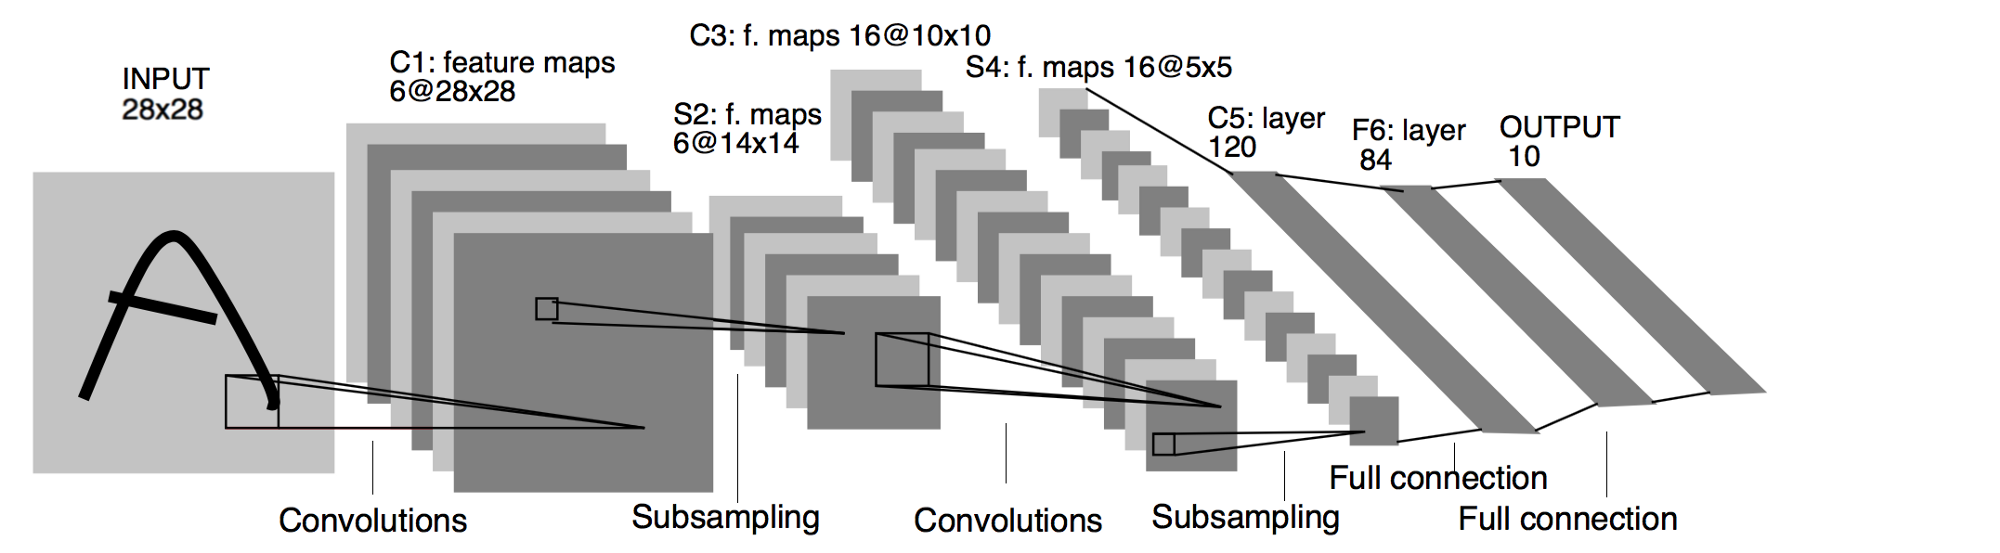
\includegraphics[scale=0.2]{hw6/images/lenet.png}
\end{center}
\caption{Architecture of LeNet 5. Adapted from the original paper of LeCun et al.}
\end{figure}



\subsection{Instructions}
\begin{itemize}
\item Read \textbf{PyTorch}'s documentation on convolution and pooling.

\item You will need to complete the missing code (marked with \#TODO) in the script provided, \textbf{\textit{lenet.py}}.  Most of the code will be the same as that in HW5 including \#TODOs of the same functions. Feel free to reuse whatever you wrote of HW5, or the code in the solution of HW5. Also feel free to modify/add any functions when necessary. \textbf{Please append your code at the end of your pdf submission.}

\item Complete the function \textbf{\textit{\_initialize\_network}} method on \textit{lenet.py} that defines the architecture of the neural network. Hint: use nn.Conv2d(), nn.AvgPool2d(), nn.MaxPool2d(), Reshape() and nn.Flatten() modules.

\item Complete the function \textbf{\textit{get\_intermediate}} method on \textit{lenet.py} that returns the intermediate outputs requried in the questions below. This will be analogous to the \textbf{\textit{layer\_features}} function of  \textbf{\textit{\_DropoutClassifier}} in HW5.



\item Train your classifiers, we provided you with beginning code in the \textbf{\textit{main}} function. (Hint: trajectories will be available in the \textbf{\textit{trajectories}} attribute of the classifier, save the weights of your classifiers so that your progress is not lost.)

\item For reference, you should be able to reach  $~63\% $ test accuracy with max pooling after $3000$ steps if you are running with given hyperparameters. Feel free to change the hyperparameters as long as the results look reasonable. 

\end{itemize}

\subsection{Expected Results}

The architecture of the version of LeNet5 we are going to implement is: 

\vspace{3mm}

\fbox{\begin{minipage}{30em}
Input image $\rightarrow$ 2D convolution with kernel size $5$, stride $1$ and no padding $\rightarrow$ ReLU $\rightarrow$ Pooling with kernel size $2$, stride $2$ and no padding $\rightarrow$  2D convolution with kernel size $5$, stride $1$ and no padding $\rightarrow$ ReLU $\rightarrow$ Pooling with kernel size $2$, stride $2$ and no padding $\rightarrow$ Fully connected linear layer $\rightarrow$ ReLU $\rightarrow$ Fully connected linear layer $\rightarrow$ ReLU $\rightarrow$ Fully connected linear layer $\rightarrow$ Output
\end{minipage}}\\
\\
Follow the original LeNet architecture in terms of the number of feature maps and the size of weights in fully connected layers.

\vspace{3mm}

Train three CNN models: $\bm{M_{avg}}$: LeNet5 with average pooling , $\bm{M_{max}}$: LeNet5 with max pooling, $\bm{M_{no}}$: LeNet5 with no pooling. Note that even if you should use the same convolution settings as the models with poolings, you may have to change the in\_features of the first fully connected layer when you define the architecture for $\bm{M_{no}}$ because the shape of the tensors will be changed. You may also have to insert operations to reshape the input tensor from $3072$ to $3 \times 32\times 32$ (use \textbf{\textit{Reshape()}} given in the code) and flatten the tensors before the fully connected linear layer (use \textbf{\textit{nn.Flatten()}}). 
\begin{enumerate}[a]

    \item (5 points) Train your classifiers (using GPU) for \textbf{3000} steps. Alternatively, you may run your algorithm for \textbf{500} steps (using CPU), in which case you will be awarded full points for the next results, but won't receive this 5 points. 
    
    
    \item (25 points) Show the final training and testing accuracy and training time for the three models. Specify the number of steps you used for training ($3000$ or $500$). You can time the entire training process including steps for computing test accuracy. Discuss the reason for the difference of training time between $\bm{M_{no}}$ and the two models with pooling.
    
    \item (20 points) For each model, display the train and test loss vs the gradient steps (only for the given display steps specified in the hyper-parameters) in the same plot. You will show three subplots, each corresponding to a model.

    \item (20 points) For each model, display the train and test accuracy vs the gradient steps (only for the given display steps specified in the hyper-parameters) in the same plot. You will show three subplots, each corresponding to a model.
    

    \item (20 points) (For $\bm{M_{avg}}$ only) Pick a sample from the CIFAR dataset, plot 1) The original image. 2) Output of the first layer (after the first convolutional layer and before ReLU). 3) Output of the second layer (after the first pooling layer and before the second convolutional layer). \\
    In particular, arrange the three plots as follows: 1)one $32 \times 32$ image. 2) six $28 \times 28$ images. 3) six $14 \times 14$ images. Compare 2) with 1), and 3) with 2). Briefly explain your observations.
    
    \item (10 points) Design a CNN model with a different architecture. Briefly explain your architecture (use the same format in 1.3 problem description). Show the final training and testing accuracy and training time for your model and compare with the best LeNet5 result. (Try to beat the LeNet5 that we provided, though we will not grade based on performance.)
    
\end{enumerate}

\end{document}